\documentclass[11pt,a4paper,twoside,openright,bachelor,english]{netthesis}
\usepackage[utf8]{inputenc}
\usepackage[section]{placeins}
\usepackage{float}
\usepackage{xcolor}
\usepackage{listings}
\lstset{basicstyle=\ttfamily,
  showstringspaces=false,
  commentstyle=\color{red},
  keywordstyle=\color{blue}
}
\usepackage{minted}
% Include common packages
% raise package limit
\usepackage{etex}

% input encoding
\usepackage[utf8]{inputenc}

% subfiles
\usepackage{subfiles}
\makeatletter
\newif\ifsubfile\subfilefalse
\@ifclassloaded{subfiles}{\subfiletrue}{\subfilefalse}
\makeatother

% fonts
\usepackage[T1]{fontenc}
\usepackage{libertine}
\usepackage[scaled=0.8]{beramono}
\usepackage[expansion,protrusion,shrink=15,stretch=15]{microtype}
% Use libertine symbols --- Dirty hack!
% Does no longer work with new libertine package
%\DeclareTextCommand{\textbullet}{T1}{\libertineGlyph{bullet}}
%\DeclareTextCommand{\textdagger}{T1}{\libertineGlyph{dagger}}
%\DeclareTextCommand{\textdaggerdbl}{T1}{\libertineGlyph{daggerdbl}}
%\DeclareTextCommand{\textasteriskcentered}{T1}{\libertineGlyph{asteriskmath}}
% Alternatively use cmsy but get rid of warnings --- Dirty hack!
%\DeclareTextCommand{\textbullet}{T1}{$\bullet$}
%\DeclareTextCommand{\textdagger}{T1}{$\dagger$}
%\DeclareTextCommand{\textdaggerdbl}{T1}{$\ddagger$}
%\DeclareTextCommand{\textasteriskcentered}{T1}{$\ast$}

% vim: set sw=4 ts=4 et tw=0 :



% tables
\usepackage{array}
\usepackage{booktabs}
\usepackage{tabularx}
\usepackage{longtable}
\usepackage{ltxtable}

% lists etc
\usepackage{cite}

% text configurations not including font
%% define a long dash
\newcommand\drule{\rule[.56ex]{\widthof{-}}{.1ex}}
\newcommand\nrule{\rule[.56ex]{\widthof{--}}{.1ex}}
\newcommand\mrule{\rule[.56ex]{\widthof{---}}{.1ex}}
\newcommand\lrule{\rule[.56ex]{1em}{.1ex}}

% reset some length
\setlength{\textfloatsep}{1.7\baselineskip plus 0.6\baselineskip minus 0.4\baselineskip}

% vim: set sw=4 ts=4 et tw=0 :



% math
\usepackage{mathtools}
\usepackage{packages/accents}
\usepackage{fixmath} % upper case Greek letters in italics.
% All mathematical definitions
% use msvsymbols package
%\usepackage{msvsymbols}

\usepackage[libertine,cmintegrals,libaltvw]{newtxmath}
\usepackage[
bb=ams,
scr=rsfs,
cal=cm
]{mathalfa}

% libertine math font stuff
\makeatletter
\DeclareMathSymbol{0}\mathalpha{operators}{"30}
\DeclareMathSymbol{1}\mathalpha{operators}{"31}
\DeclareMathSymbol{2}\mathalpha{operators}{"32}
\DeclareMathSymbol{3}\mathalpha{operators}{"33}
\DeclareMathSymbol{4}\mathalpha{operators}{"34}
\DeclareMathSymbol{5}\mathalpha{operators}{"35}
\DeclareMathSymbol{6}\mathalpha{operators}{"36}
\DeclareMathSymbol{7}\mathalpha{operators}{"37}
\DeclareMathSymbol{8}\mathalpha{operators}{"38}
\DeclareMathSymbol{9}\mathalpha{operators}{"39}
\makeatother

%% math alphabet fonts
\DeclareSymbolFont{nxlmibit}{OML}{nxlmi}{bx}{it}
\DeclareSymbolFontAlphabet{\mathbit}{nxlmibit}
%FIMXE: the first package seems to cause an \if\fi bug
%\DeclareSymbolFont{libertineplus}{T1}{ntxrx}{m}{n}
%\DeclareMathSymbol{+}{\mathbin}{libertineplus}{43}

\newcommand\showmathalphabet{\noindent\begin{tabular}{ll}
    mathnormal  & $abcdefghijklmnopqrstuvwxyz$\\
                & $ABCDEFGHIJKLMNOPQRSTUVWXYZ$\\
    mathrm      & $\mathrm{abcdefghijklmnopqrstuvwxyz}$\\
                & $\mathrm{ABCDEFGHIJKLMNOPQRSTUVWXYZ}$\\
%    mathit      & $\mathit{abcdefghijklmnopqrstuvwxyz}$\\
%                & $\mathit{ABCDEFGHIJKLMNOPQRSTUVWXYZ}$\\
    mathbf      & $\mathbf{abcdefghijklmnopqrstuvwxyz}$\\
                & $\mathbf{ABCDEFGHIJKLMNOPQRSTUVWXYZ}$\\
    mathbit     & $\mathbit{abcdefghijklmnopqrstuvwxyz}$\\
                & $\mathbit{ABCDEFGHIJKLMNOPQRSTUVWXYZ}$\\
%    mathfrak    & $\mathfrak{abcdefghijklmnopqrstuvwxyz}$\\
%                & $\mathfrak{ABCDEFGHIJKLMNOPQRSTUVWXYZ}$\\
    mathcal     & $\mathcal{ABCDEFGHIJKLMNOPQRSTUVWXYZ}$\\
%    mathscr     & $\mathscr{ABCDEFGHIJKLMNOPQRSTUVWXYZ}$\\
%    matheus     & $\matheus{ABCDEFGHIJKLMNOPQRSTUVWXYZ}$\\
\end{tabular}}

% vim: set sw=4 ts=4 et tw=0 :



% theorems
%\input{pream/TheoremStyles.tex}

% listings
\usepackage{listings}

% drawing and graphics
\usepackage{packages/tumcolors}
\usepackage{tikz}
\input{pream/TikzStyles.tex}
\usepackage{packages/moeptikz}

% IEEE tools for tweaking bib style
\usepackage{packages/IEEEtrantools}

% enable links
\usepackage[colorlinks=false,pdfborder={0 0 0}]{hyperref}
\newcommand\toc{\relax}

% pgfplots
\usepackage{pgfplots}
\pgfplotsset{compat=newest}
\pgfplotsset{colormap={moepcolormap}{[1cm] color(0cm)=(black!60) color(5cm)=(black!1)}}
%\pgfplotsset{colormap={moepcolormap}{[1cm] color(0cm)=(TUMDarkerBlue) color(1cm)=(TUMLighterBlue) color(2cm)=(TUMGreen) color(3cm)=(TUMBeamerYellow) color(4cm)=(TUMOrange) color(5cm)=(I8LogoRed)}}






% hyphenation
\hyphenation{op-ti-cal net-work net-works semi-con-duc-tor tech-nique tech-niques}


% Needed for Bachelor's theses, Master's theses and IDP
\titlegerman{Leistungsanalyse der Funktionen von Middleboxes}
\titleenglish{Performance Analysis of Middlebox Functionality}
\submitteddate{\today}
\author{Simon Sternsdorf}
\supervisor{\NEThead}
\advisor{Florian Wohlfart}

% Additionally needed for dissertations
\committeechair{}
\committeeexaminers{}{}{}
\accepteddate{}


\begin{document}%

% Makes sure that same author names are not replaced by dahes
\bstctlcite{IEEEexample:BSTcontrol}

\pagenumbering{gobble}
\maketitle%


\subfile{include/abstract.tex}


\pagenumbering{Roman}%

{\tableofcontents}
{\listoffigures}
{\listoftables}

\cleardoublepage

\pagenumbering{arabic}

\chapter{Introduction}

\section{Motivation}
Middleboxes are mediating devices used by both End-user Internet Service Providers (ISPs) and normal home users. The requirements ISPs have for middleboxes are of course vastly different from the requirements of private users. Thus the implementations differs greatly as well. Middleboxes for home users do not have high performance requirements. They conduct mostly very simple tasks for a low amount of devices. This is changing of course, as more and more web-enabled devices are used in modern households. 
Still the required performance is low in contrast to at an ISP for example. Especially carrier grade network address translation is used to provide ipv4 connectivity for mobile phones, since IPv4 addresses are getting rare \cite{A10}. The middleboxes used are mostly implemented in hardware, which has assets and drawbacks. Those drawbacks are significant. 
middleboxes specifically produced for ISPs are expensiv both in acquisition and maintainance, also they usually have to be replaced to introduce new features \cite{WhiteP}. Also they are difficult to scale with higher or lower demand. All these problems are avoidable through network function virtualization. And the long-term plan is indeed to replace these hardware middleboxes with all-purpose hardware that is cheap and easily replaceable \cite{Click}. The networking functions would be implemented in software. 7 of the worlds largest telecoms network operators are in an standards group for virtualization of network functions. So the topic is already being discussed in ISPs \cite{NetDis} 



\section{Goal of the thesis}
The goal of this thesis is to test different software middlebox implementations. We will install different middlebox implementations in our testbed. Then we will test the packet processing capability, try to find bottlenecks for the performance when processing packets. We will evaluate our results. 
Additionally we want to evaluate if software middleboxes are competitive with hardware implemented middleboxes and could replace them in the foreseeable future. 

\section{Outline}

The thesis reads as follows. The second chapter introduces the theoretical concept of NAT and a NAT model which we used in our tests. Also it defines performance testing. Additionally the Data Plane Development Kit is introduced, DPDK. The third chapter informs the reader about the general idea behind our tests. Further it presents the software used for the tests. This includes the software running on the device under test, as well as the software used to run the tests. It explains the methodological approach used in this thesis. Here it explains the setup for the experiment. In chapter 4 are the collected results of the Firewall and NAT tests with a brief analysis of the result. Finally chapter 5 summarizes the outcome and gives possible future works of this thesis. 

\chapter{Background}

This chapter gives a overview over network address translation and the NAT model we will assume in this thesis. Also it will explain our approach to performance testing. Finally the chapter outlines the Data Plane Development Kit, developed by Intel \cite{DPDKOv}.

\section{NAT}

Network address translation NAT was first described 1993 and written into RFC 3022 \cite{RFC3022} in 2001. It was proposed as an temporary solution for the shortage of IPv4 addresses. It should slow down the need for IPv4 addresses of private customers and businesses \cite{bonaventure2011computer}. It does this by working as a connector between two different networks with different IPv4 address spaces. Mostly it translates between the address space of the Internet and a private network. Since NAT is used so broadly it is one of the most common middleboxes. $\newline$
NAT in private households is in many instances implemented directly in the router. The home ususally only gets one IPv4 address from its ISP. The router then interconnects the home network to the Internet via an ISP. It translates the private IP addresses of the home network to enable them to share the single IPv4 address \cite{bonaventure2011computer}[Page 168]. In corporate networks it basically fulfills the same purpose. The main difference is that the border router manages multiple public IPv4 addresses and manages the correct translation between them and the private IPv4 addresses in the private network. 
Here we see the simple version with only one public IPv4 address.

\begin{figure}[h]
\centering
{\includegraphics[width=.75\columnwidth]{figures/NATPrivate}} \quad
\caption[A simple NAT with one public IPv4 address]{ A simple NAT with one public IPv4 address \cite{bonaventure2011computer}[Page 168]}
\label{fig:NATPrivate}
\end{figure}

A NAT middlebox manages the translation between the different IPv4 address spaces. To achieve this the middlebox has to save a mapping of the private IP addresses to the public ones. In the simplest imaginable case we have as many public IPv4 addresses as we have private ones. In that case the mapping is simply a bijection. When the NAT middlebox receives a packet from a new private IP S in the internal network it maps it to a not used public IP from its address pool. This mapping is saved. To translate the packet the NAT middlebox has to : $\newline$
\begin{enumerate}

\item Replace the original source IP from the packet with the mapped public IP
\item Completely recompute the IP header checksum, as not only the Time To Live header field changes, but also the source IP header field \cite{tanenbaum1996computer}[Page 435]
\item Recompute the checksum in the TCP or UDP header if existent. The checksum of these protocols computes the checksum over the whole packet

\end{enumerate} 

When an answer from the Internet arrives the NAT middlebox has to to the same process only with replacing the destination IP address with the source address of the private host. This is done with the same mapping. Afterwards the packet is forwarded to the host in the private network. $\newline$
In the realistic case where we have less public IP addresses then private ones the translation occurs over the IP and the port number. An NAT middlebox that uses this translation method maps the internal IP and the internally used port number of the TCP or UDP packet to a public IP from the IP pool available to the NAT middlebox and the first available port number \cite{bonaventure2011computer}[Page 169]. The entries in the mapping table are removed by the system after either the TCP connection is closed or the connection is idle for a longer time. Here the NAT middlebox functions similarly to a stateful firewall, which will become important later. 
When the NAT middlebox has to handle packets from the Internet, it looks up a mapping from its state table for the destination IP address and the destination port. If a matching mapping exists the packet is translated accordingly and forwarded to the matching internal host. If no such mapping exists the packet gets discarded, as there is no way to determine the correct internal host. $\newline$
NAT has two main disadvantages: Opening TCP connections from the Internet to an internal network is very difficult. This means that for example FTP users behind NAT have problems. In active mode, the FTP client first establishes a control connection to the server.After that the client listens on a random port for the incoming data connection from the server. If the client sits behind a NAT this connection will not work \cite{FTP}.$\newline$
The other disadvantage is that NAT breaks the end- to end transparency of the IP layer and the application layer. This problem occurs when the IP address is used in the application layer, as the NAT only replaces the IP in the IP header. This can be avoided with an Application Level Gateway installed at the NAT. However it is not feasible to install an an ALG for every application that relies on the IP in layer 7 \cite{bonaventure2011computer}[Page 169]. $\newline$
IPv6 would make NAT middleboxes obsolete, although some people argue NAT still has some use cases when only IPv6 is used. This is discussed in RFC 5902 \cite{RFC5902}. With IPv6 enough addresses are available to give each device a unique global IP. 

\section{NAT model} \label{NATmodel}

This section is about the NAT model we will use in this thesis and why it is important for the performance tests we did. This model is based on the basic concept of how a NAT middlebox works. Roughly speaking we will split up NAT in different components. This way we can get an better understanding of which part of the NAT is actually responsible for how much of the time we need to forward a packet. $\newline$ 
In the model the NAT middlebox performs 3 tasks excluding the sheer forwarding of the packet: 
\begin{itemize}
\item Parse the packet. This means it has to check the IP header for the source  and destination IP address and also the port numbers. Here the NAT compares to a stateless firewall, which has to do the same things. 
\item Holding a state. The NAT middlebox has to remember the mapping it created for a connection. This is similar to the state-holding of a stateful firewall. A stateful firewall tracks the state of every single TCP connection that goes through it and keeps a 5-tuple for every open connection. This 5-tuple persists of the source and destination IP, the source and destination port and the protocol used for the connection. This makes 5-tuple unique to its connection \cite{bonaventure2011computer}[Page 167].
\item Rewriting either the source or destination IP address, and rewriting the source or destination port respectively. When the NAT middlebox has to translate the packet to forward it either to the Internet or the private network it has to replace the right IP address and the right port. 
\end{itemize}
$\newline$
This simple model for a NAT middlebox will us help hopefully to determinate the different factors that influence the performance of the NAT middlebox.  


\section{Performance testing}

Performance testing is the term that designates a testing technique to determine how a system reacts in term of steadiness and amenability under different amounts of load. 
With this testing we can learn about the quality of our system and its attributes \cite{TutPer}. There are different forms of performance testing. $\newline$
\begin{itemize}

\item Load testing. Load testing is a very simple form of performance testing where the system is tested under specific work loads. All the parts of the system get monitored. With this one can predict how the system will react in the future under concrete work loads.

\item Soak testing. Here the system is monitored under an continuous load. The load is set to the excepted average work load the system has to handle. With this testing the endurance of the system is determined. Critical parts like the memory of the system are monitored to find possible performance issues or errors under uninterrupted use.

\item Spike testing. As the name suggests this testing revolves around a sudden spike of new users in the system. This is simulated by suddenly increasing the number of virtual users and monitoring the system. This test shows if a system can manage such a strong spike of new users and also if the system can handle the continuous workload that comes with a bigger user base.

\item Stress testing. Stress testing is used to determine the maximum workload a system can handle. Also it shows how a system performs with a workload well above its limits. This is done by monitoring the system and increasing the workload until a part of the system fails or cannot complete the work correctly.

\end{itemize}
$\newline$

We will take a closer look at stress testing since it is the main form of performance testing we used here. In a stress test the condition of our system is progressively worsened until the performance is too low as that we could use the system or the system fails entirely. To exactly determine which element of the system failed we have to have indivisual stressors that are varied, and see which effect they have. Stress testing can often take a long time, but is really important to determine the degree of graceful degradation of a system. Graceful degradation describes the capability of a system to still be somewhat operational even under extreme circumstances. This is important for critical systems which always have to be operational \cite{Stress}. 



\section{Data Plane Development Kit}

The Intel Data Plane Development Kit, Intel DPDK, is a group of programming libraries available in source code. These libraries enable faster basic data plane functions on Intel processors. These lbraries are especially designed to optimize the packet processing capabilities on IA processors. These are processors from the Xeon series. These libraries allow for fast implementation of packet forwarding functions \cite{DPDKEx}.
The most important DPDK elements can be seen in \ref{fig:DPDKEx} 
\begin{figure}[h]
\centering
{\includegraphics[width=.75\columnwidth]{figures/IntelDPDK}} \quad
\caption[ Intel® Data Plane Development Kit]{ Intel® Data Plane Development Kit \cite{DPDKEx}}
\label{fig:DPDKEx}
\end{figure}

This shows the different DPDK libraries for buffer management, queue management, packet flow classification and poll mode drivers for different network interface cards. DPDK provides a model with a low overhead to enable a optimal data plane performance. It includes an Environment Abstraction Layer, which includes platform specific code. This simplifies application porting \cite{DPDKEx}. $\newline$
The buffer management includes the DPDK Memory Manager, which allocates pools of objects in the memory. This is realized through a ring to store free objects, which accelerates the whole process. Additionally the DPDK Buffer Manager reserves buffers with a fixed size. This additionally accelerates the system, as we no longer have to constantly allocate new buffers or free buffers which are no longer in use. $\newline$
The packet flow classification includes the Intel DPDK Flow Classifier, which uses Streaming SIMD Extensions to speed up the process of placing packets in the right flow to get them processed. This additionally improves the throughput of the system \cite{DPDKEx}.
$\newline$
The poll drivers included in DPDK work for Gigabit Ethernet and 10 Gigabit Ethernet and work with asynchronous signal mechanisms. This improves the performance for pipe-lining packets. $\newline$
Since 2013 exists dpdk.org \cite{DPDKOv}, a Open Source Project founded by 6WIND \cite{DPDKEx}. Through this project source code, a documentation and example applications are available. This code is pretty much up-to date with the Intel DPDK releases and provides high processing-performance. The open-source project sees a lot of interest and is used already in several big projects and of course many smaller programs. One of them is for example MoonGen, which we will discuss in the Methodology chapter. $\newline$ 
As a short conclusion in DPDK, we can see that DPDK could be vital to accelerate packet processing and handling in software middleboxes. It has great capabilities and sees a lot of ongoing development from Intel \cite{DPDKEx}.


\chapter{Methodology}

Before we can start testing the performance of a software middlebox of our choice, we have to decide on test parameters. This involves how we should conduct the measurements, what we want to measure, how the measurements should look like etc. For example we have to decide on a load generator, what kind of test environment, how we want to collect and visualize the data that we derive, and most importantly the middlebox software we want to survey. 
$\newline$
In this chapter we discuss the research methodology and its design and implementation.

\section{General Idea}

To test a software middlebox we defined a specific test setup which will help us derive the most precise results. This means we will be able to determine in which areas the middlebox software is performant and which properties of our traffic are most influential on this performance. The exact setup will be described in the following section. $\newline$
The short abstract of it is: We will conduct black box tests of a middlebox software we installed on the DUT, the device under test. This DUT is connected to our testserver. This testserver runs a load generator to stress test our middlebox software. $\newline$

\begin{figure}[H]
\centering
{\includegraphics[width=.85\columnwidth]{figures/Testsetup}} \quad
\caption[Our testsetup ]{ Testsetup }
\label{fig:Testsetup}
\end{figure}
$\newline$

\subsection{Black box testing}

Black box testing is an important part of testing software. At its core it is used to analyze software without knowledge or reference to the internal working of the software. This enables us to test the functionality of the software with basically no consideration of the internal processes of the software \cite{khan2010different}. 

\begin{figure}[H]
\centering
{\includegraphics[width=.65\columnwidth]{figures/black_box_testing}} \quad
\caption[Working process of Black box testing ]{Working process of Black box testing \cite{BlackboxWiki}}
\label{fig:BlackBox}
\end{figure}

$\newline$
This method has following advantages for the tester:
\begin{itemize}

\item The tester does not need to know how the software that they test is implemented. This means the tester does not have to be a software developer. 

\item The tester can be someone independent from the developer, removing possible bias from the tests and how the are conducted. This means there exists no "bond" between the tester and the code. 

\item The perception for the tester is very simple

\end{itemize} 

Some disadvantages of blackbox testing for our case include: 
\begin{itemize}

\item Not all the possible inputs can be tested. This means for the middlebox for example, we can't test every single possible combination of flow length, packet size and transmit rate.

\item When tests throw errors it is harder to understand and determine why this certain test failed, as we can't just look inside the running DUT.\cite{khan2010different}

\end{itemize}



\subsection{Software}

For the tests we need software to implement and run the DUT and software to generate and record traffic. For one we need the middlebox software. As explaned in \ref{NATmodel} we want to implement and understand NAT in different states. This means our software middlebox needs to be very flexible. As our main features we need a stateless firewall and the NAT functionality. The software needs to run on our hardware under Linux. Preferably the software should use DPDK or similar software to increase the performance of the packet forwarding. Otherwise if the software uses the Linux Kernel it should at least have the option to use DPDK in the future. To test the performance of the DUT we need a load generator. The load generator needs to generate enough load to saturate a 10 gigabit Ethernet connection, as our two servers are connected with 10 gigabit Ethernet. Technically the load generator only needs to generate more load than the DUT can handle. As we do not know how much middlebox software on our server can handle we are aiming for the maximum load possible. Also our load generator must be able to accurately measure the latency of our packets. Important for the tests are the different metrics we can define with the load generator. To fully test the middlebox we need to be able to change the metrics of our packet stream very freely. This includes the packet sizes, different ports, different IP addresses and different transmit rates.

%%Potential: Testframework


\section{Test Methodology}

This section introduces the specific software we chose for the testsetup. We will discuss the advantages and disadvantages of the choices we made. Also we will explain the experimental setup we arranged to test the middlebox software. A great deal of the setup was already established by the testbed. 


\subsection{Experimental Setup}

To assure that the results were reliable and reproducible, we conducted the tests on one system, here the system tallinn. This means we used the same two servers for our experiments.  
$\newline$ 
The Hardware of the system was: 
\begin{itemize}

\item CPU: Intel(R) Xeon(R) CPU E31230 @ 3.20GHz

\item Number of CPUs: 1
\item Memory: 16 GB
\item Mainboard: X9SCL/X9SCM
\item NICs: 2x Intel X540 (1x X540-T2)


\end{itemize}

As operating system Debian 8.9 "Jessie" was used, as it was newest Debian system at the time. It was not further modified in any way. Debian was already preconfigured in the testbed for easy install. By using Debian I was able to automate most of the setup process for the device under test and the load server. The servers were connected as can be seen in \ref{fig:Testsetup} with 10 Gbit cables between them. On one server I installed the load generator on the other on the middlebox software which I configured for the tests. The following sections will explain the used programs in more detail. 

\subsection{MoonGen Traffic Generator}

\subsubsection{Advantages and disadvantages}

MoonGen is a software-based traffic generator that can saturate 10 Gbit Ethernet easily while using a very special approach for measuring the latency of the packets. MoonGen was selected out of a few possible candidates mainly because of its flexibility. Most packet generators are either very complicated or have no good performance. The tested alternatives to MoonGen were either very complicated to set up and run, or had a bad performance \cite{emmerich2015moongen}. MoonGen has 4 major advantages over the rest for my use case: $\newline$
\begin{itemize}

\item MoonGen is completely implemented in software and can run on a lot of commodity CPUs. This is achieved through its implementation on top of DPDK, the packet processing framework. The only requirement for our hardware is that DPDK supports it and that it offers support for the time stamping and rate control. 

\item Is very flexible, as the packet generator logic is written in Lua scripts. These scripts are very user friendly and can be completely modified. In this specific case LUA-JIT was used as its performance is suited for high speed packet processing. 

\item Is able to saturate multiple 10 Gbit Ethernet interfaces with minimum size packets. This advantage was not really necessary for this specific test setup as we only needed to saturate one interface. But the good performance was still noticeable. 

\item MoonGen allows to time stamp very accurately and building on that very good rate control. This point will be further explained below. 

\end{itemize}

One disadvantage of MoonGen is that it currently only supports UDP packets for layer 3 latency measurements. MoonGen is not able to understand the TCP stack and therefore cannot establish a TCP connection. This was important when testing the middlebox software mOS, which will be talked about later. 

\subsubsection{Closer Look: Hardware timestamping }

The type of hardware timestamping in MoonGen is very unique. It utilizes the IEEE 1588 Precision Time Protocol (PTP), which is used for clock synchronization across networks. It is supported by a large variety of NICs. PTP is either used as a protocol on layer 3 or on top of UDP on layer 4. This hardware timestamping works at the moment with the Intel 82580 GbE, the 82599 and X540 10 GbE chips. These NICs support the timestamping with PTP Ethernet and UDP. Moongen configures them to only recognize PTP packets with a specific first byte in their header. The second byte represents the PTP version number. The other PTP fields are not used and can contain any value. This allows MoonGen to measure the latency of any packet. $\newline$ 
All timestamps fro recieved and transmitted packets get saved in a special register directliy on the NIC. This register has to be read out before the next packet can be timestamped. Some NICs also support the prepending of timestamps of new packets to the buffer. With these timestamping mechanisms MoonGen can reach a precision of 64 nanoseconds on a 10GbE link \cite{emmerich2015moongen}.


\subsection{mOS} \label{mOSBegin}
This section will explain why mOS was chosen initially as a middlebox candidate and why it wasn't usable for this paper. $\newline \newline$

\subsubsection{Approach of mOS}
Middlebox OS is a reusable networking stack, which enables stateful flow processing. mOS provides an API for developers to programm middlebox applications on top of mOS. This enables the developers to concentrate on the important logic of the middlebox and the top level rather than the finicky low-level packet processing. This means the applications would be more consistent and easier modifiable. Also it prevents the introduction of new errors when the programmer has to implement the complex flow mechanisms from scratch. Most importantly, mOS promised a consistent and high performance even though it essentially provides a software middlebox. The developers of mOS promised an "efficient event system that scales to monitoring millions of concurrent flow events" \cite{jamshed2017mos}[Abstract]. $\newline$
The API of mOS includes programming presets that introduce the programmer to flow-events. Flow-events are operations the middlebox can fulfill which are definable by the user. This makes mOS very easy to deploy and to adjust to your networking situation. 

\begin{figure}[H]
\centering
{\includegraphics[width=.85\columnwidth]{figures/mOSFlow}} \quad
\caption[ mOS/Application Interaction]{ mOS/Application Interaction \cite{jamshed2017mos}  }
\label{fig:mOSFlow}
\end{figure}

$\newline$
mOS enables easier development by providing a monitoring socket for developers as can be seen in Figure \ref{fig:mOSFlow}.  This enables the developer to see exactly what happens with a single TCP flow running through the middlebox. Additionally, mOS includes scalable monitoring. Scalable monitoring helps to reduce the overhead that gets induced when tracking so many different flows. This reduces the memory usage of mOS for example for dynamic event registration and deregistration. $\newline$ Also developers can enable and disable event generation for flows and reduce recourse usage this way. By deactivating the tracking of unnessesary properties if the flows mOS reduces the overall system load. This leads to higher performance and reduces waste of CPU cycles \cite{jamshed2017mos}. $\newline$

\begin{figure}[H]
\centering
{\includegraphics[width=.85\columnwidth]{figures/mOSThread}} \quad
\caption[ mOS application threading model]{ mOS application threading model \cite{jamshed2017mos}  }
\label{fig:mOSThread}
\end{figure}
$\newline$
To increase performance, mOS uses a shared-nothing parallel-processing threading model. This model works especially great on modern multi-core CPUs. As you can see in Figure \ref{fig:mOSThread}, mOS initializes n threads each bound to a CPU core. Each of these threads handles flows using symmetric receive-side scaling (S-RSS). All packets that are associated to the same connection are mapped by S-RSS to the same RX queue in the NIC. This enables the forwarding of packets with line rate, as all the packet classification is done in hardware by the NIC itself which is very performant. This also enables the shared-nothing parallel-processing threading model, as every connection is handled by one thread. This enables mOS to avoid inter-clock locks and cache interferences \cite{jamshed2017mos}.   
$\newline$

mOS relies on kernel-level NIC drivers to forward the packets into the symmetric RSS. DPDK or PCAP are supported as default I/O module. $\newline$

\begin{figure}[H]
\centering
{\includegraphics[page=11,width=.65\columnwidth]{figures/mOSDPDKSummit}} \quad
\caption[ mOS shared-Nothing Parallel Architecture]{mOS shared-Nothing Parallel Architecture \cite{mOSStack}  }
\label{fig:mOSStack}
\end{figure}

Figure \ref{fig:mOSStack} displays the function of the NIC-drivers. mOS reads multiple packets at once from the incoming packet stream. Packets are processed by the run-to-completion model. This model allows all threads in an application to use a single stack, which of course has as a consequence that threads cannot block or wait on events. But threads can be initialized by events \cite{belay2014ix}. The use of this model is ideal for applications with huge importance on events and real-time applications. The threads are very keen handling processes with an high frequency of interrupts. 

$\newline$
We initially chose mOS as our middlebox test candidate because it promised great performance with high flexibility. Since it is based on mTCP it can work with the complete TCP stack and we planned to make further tests with the TCP stack. In its repository mOS also includes sample applications. These seemed very useful, as a NAT application and a stateless firewall application were given. With the simple expression language mOS uses for the applications they seemed easily modifiable. Also the testing of the sample applications could get us some insight in how the middlebox applications performed in our testbed with our load generator in general. mOS can run on commodity hardware. The hardware in our testbed is not exactly the same as the developers used in their paper but our hardware fulfills the requirements given for mOS.  This made mOS a good candidate for our tests. 



\subsubsection{Setup in the testbed}

To set up the base mOS on one of the servers in the testbed I followed the documentation of the mOS developers. This involved installing several packages of the Debian repositories as well as installing DPDK with all its dependencies. We decided to use mOS compiled with the DPDK library and not with the PCAP library. We made this decision based on the data provided by the mOS developers, which promised a better performance with the DPDK libraries \cite{mOSStack}. Afterwards I compiled mOS with DPDK. This involved setting up hugepages. 1024 2 MB pages were used. Afterwards the Ethernet devices connected to the load server were loaded and bound to the IGB\_UIO module. This module is a wrapper module. It sits on top of the UIO module of the linux kernel and allows for the DPDK drivers in the user space to access the registers on the NICs \cite{mOSDoc}. 
$\newline$
Because of the structure of our testbed mOS was used in inline mode. 

$\newline$
\begin{figure}[H]
\centering
{\includegraphics[width=.65\columnwidth]{figures/midstat_inline}} \quad
\caption[ mOS inline model]{ mOS inline model \cite{mOSDoc}  }
\label{fig:mOSInline}
\end{figure}
$\newline$

In inline-mode mOS runs on a separate host that connects two data networks as can be seen in Figure \ref{fig:mOSInline}. For this test setup the two data networks are actually two interfaces of the load server. Here in \ref{fig:mOSInline} the chosen mOS application is Middlebox Stats (midstat). It is a basic monitoring application. Because of the position of the application all the traffic between the data networks goes through it, thus enabling the application to monitor, drop or manipulate the traffic in both directions. 
With this mode we basically simulate that one interface of our load server is an internal network and the other one is an big outside network like the internet. The mOS NAT application in between would replace the IP address of packets coming from the internal network with the public IP it got assigned \cite{mOSDoc}.
$\newline$
After making sure that the IP addresses of the two interfaces on the DUT were unassigned and adjusting the mOS configuration file for the application we wanted to run the setup was finished. We started by using the sample applications that are included with mOS, mostly the NAT application and the simple\_firewall. Although these applications do not depict the whole range of possibilities of mOS, they provided the ground basics we wanted to measure. 


\subsubsection{Problems}
As stated before in section \ref{mOSBegin}, mOS had 2 main problems during the setup and when the applications were running. We had some minor problems as well but were able to fix them. We put quite some effort into fixing these problems (including contacting the mOS developers), but we were unable to fix these problems with a reasonable amount of work as part of this thesis. This sadly meant we had to drop mOS \cite{mOSGit}.
$\newline$
The first issue already occurred when starting the example applications. When starting the NAT or the midstat application via the command line interface  a parameter can be given for the amount of cores the application can use. The simple\_firewall just uses all available cores per default. Our DUT has a CPU with 4 physical cores and 8 threads. But when using all 8 virtual cores the Linux machine ran Out of Memory (OOM), which resulted in terminating the application. This had as result that we could only use the applications with 6 virtual cores, which we had to hard-code into the simple\_firewall application. We tried to allocate even less cores to maybe reduce possible errors, but encountered problems. With 3 or less cores the applications would start normal and their monitoring seemed to work fine. But they would not process or even simply forward any incoming packets. So we settled with 6 cores for the applications. $\newline \newline $
The second and much bigger issue we only discovered after already setting up and testing for quite some time. When measuring the latency using MoonGen the results appeared really promising. With 4 flows and minimum packet size, by using the full line rate, we achieved a respectable throughput. The middlebox couldn't however handle a higher flow number. The amount of flows depended on the amount of virtual cores we assigned to the mOS application. With 6 cores the most amount of flows the mOS application managed was 23. This was consistent with every application we tested, the midstat application, the NAT application and the simple\_firewall. With more than 23 flows, the system would "soft crash", as it would still run on the system and the monitoring would still update itself. But the system no longer forwarded any more packets, even after switching again to a lower amount of flows.  
This number of flows also depended on the packet size and the transmit rate we configured in MoonGen. A bigger packet size and/or a lower transmit rate make a higher number of flows possible. But even with packet sizes as big as 1500 bytes the amount of possible flows would not go over 1000. 1500 byte is the Maximum Transmission Unit (MTU) for Ethernet. This implied huge limitations for the software as a whole. A software middlebox, even in a private household, has to be able to handle more than 23 flows. With the amount of Internet of Things devices a modern household has, this number can be easily exceeded. Since every device has a private IP address all these IP addresses need to be translated by the NAT most households with included in a router. A middlebox for an ISP or a bigger company would need to be able to handle multiple thousand if not ten thousand flows at once. $\newline$ 
This also had implications for the tests we could conduct with mOS. This meant we would have to remove one variable from our tests. And one that was particular interesting, as the amount of different flows arriving in a short time span is the big difference between middleboxes in private households and middleboxes used by ISPs. $\newline \newline$
All in all this meant mOS would have severely limited our study as a software middlebox for this paper. Even though mOS was an interesting system with a new approach to the software middlebox, the limitations with the flow amount were severe and the tests of this paper would not have been possible in a meaningful way with mOs. 

\subsection{Open VSwitch}
After mOs had proven insufficient, we moved on to the next candidate middlebox software, Open VSwitch (OVS).
Open VSwitch is the middlebox software we settled on using. In it's core, OVS is a virtual switch. Hypervisors need to bridge traffic between VMs and the outside network interface. When the hypervisor is Linux-based this usually means using the standard Linux bridge, which is the L2-switch that is built into Linux. This switch is mostly reliable, but has problems concerning multi-server virtualization and speed. Here Open VSWitch presents as a more useful and better performing solution than the Linux bridge \cite{OpenVSwitchWhy} . $\newline$ Open VSwitch is licensed under the Apache open source license \cite{OVSLicense} . Open VSwitch supports most of the standard management interfaces and protocols. It works in the most commonly used virtualization environments like Xen, KVM and Virtualbox as well in virtual management systems. It is mostly used to virtualize multiple servers at once \cite{pothuraju2016measuring}. 
$\newline$
\begin{figure}[H]
\centering
{\includegraphics[width=.85\columnwidth]{figures/OpenVSwitch}} \quad
\caption[ Distributed OpenVSwitch ]{ Distributed OpenVSwitch \cite{OpenVSwitchNVFI}  }
\label{fig:OpenVSwitch}
\end{figure}

Open VSwitch enables logical abstraction between different virtual machines and handles the offloading to the actual switching hardware. To control this OVS lies on top of the virtualization layer of the hypervisor and provides interfaces to the virtual machines. $\newline$
The virtual machines contain virtual interfaces. These enable communication between the VMs running on the same hypervisor or connected in the same virtual network and forward the traffic to the actual network interface of the machine. Here OVS acts as a bridge between the VMs and the physical interfaces. In short it interconnects the virtual interfaces with the physical interfaces \cite{pothuraju2016measuring}. 

\subsubsection{Advantages of Open VSwitch}

Open VSwitch is used as an alternative to the basic Linux bridge for modern hypervisors. OVS has some clearcut advantages over the classic Linux bridge mostly in terms of performance. 
\begin{itemize}

\item Fast self-regulation when the network environment changes, realized through sFlow and Netflow. 

\item Very easy configuration and automation of network systems. Slow and fast network states can be migrated between instances. 

\item OVS can manipulate packets to enable a better administration of different flows. This means especially changing tags in packets or reordering them. This can speed up the network processes \cite{pothuraju2016measuring} .

\end{itemize}


\subsubsection{OVS with DPDK support}

Open VSwitch forwards packets over the kernel data path, which means it uses the standard Linux kernel. This method divides the packet processing in a slow path and a fast path. The fast path matches incoming packets on a flowtable to determine the forwarding rule for the specific packet. The first packet from a new flow does not match anything in the flow table and is sent via the slow path in the user space daemon. After the user space has processed the packet, the user space daemon gets the information for the flow table from him and includes them in the current flow table. All subsequent packets of the flow can be handled via the fast path again. $\newline$
By using this approach native OVS is a lot faster than normal user space packet forwarding. Still, the context switching required for new flows limits the realistically achievable throughput. This means native OVS is not feasible for use cases were a high throuhgput is mandatory \cite{OpenVSwitchDPDK}.  $\newline$
With the use of DPDK in OVS, the slow path can make use of the Poll Mode Drivers. These enable the fast forwarding of packets from the user space to the interfaces, without the need for extra interrupt handling of the kernel. This means we essentially bypassing the whole kernel network stack. By incorporating DPDK with the Poll Mode Driver in Open VSwitch the slow path essentially becomes the fast path, as in both cases the path of the packet is the same. $\newline$
\begin{figure}[H]
\centering
{\includegraphics[width=.80\columnwidth]{figures/OVSDPDK}} \quad
\caption[ OpenVSwitch with and without DPDK]{OpenVSwitch with and without DPDK \cite{OpenVSwitchDPDK}  }
\label{fig:OpenVSwitchDPDK}
\end{figure}

This can be see in \ref{fig:OpenVSwitchDPDK}. The NAT extension of OVS does not support DPDK just yet. The support is announced for version 2.7 which will probably be released in 2018 \cite{OVSNATDPDK} . %%Possible Extension from Intel Page

\subsubsection{Connection tracking in OVS}
The connection tracking module in OVS is relatively new. Originally OVS only supported stateless matching. That made the implementation of firewalls quite difficult. For example does OVS support the match on TCP flags. This enables a fast stateless firewall by matching on TCP SYN and TYP ACK flags. But UDP traffic and traffic with ACK flag set gets through the firewall unhampered. Another way to set up a firewall in OVS is with a learn action which builds a new flow in the reverse direction. But this has to direct new flows once again through the user space which reduces the speed significantly \cite{OVSconntrack}. $\newline$
With OVS 2.5 a connection tracking module was introduced. It supports the stateful tracking of flows as well as application-level gateways for different protocols like ftp. 

\begin{figure}[H]
\centering
{\includegraphics[page=6,width=.90\columnwidth]{figures/OVSconntrack}} \quad
\caption[ OpenVSwitch with the conntrack module]{OpenVSwitch with the conntrack module \cite{OVSconntrack}  }
\label{fig:OpenVSwitchconntrack}
\end{figure}

As you can see in Figure \ref{fig:OpenVSwitchconntrack} the new conntrack module allows us to create and update CT entries without the need to go through the user space. This greatly improves the performance of the action. With the new module come different extensions for OpenFlow, which allow us to send a new connection to conntrack to start tracking it. The extension match on fields in the first packet. $\newline \newline$
This stateful matching enables a lot of other applications for OVS, for example also stateful NAT. As of now, OVS supports DNAT and SNAT. At the moment this uses the NAT features of netfilter, which is the packet filtering framework in Linux. With netfilter the OVS NAT supports port range and address range mappings with different mapping modes. 
This means the stateful NAT in OVS has all the features we expect from a middlebox NAT. 
\begin{figure}[H]
\centering
{\includegraphics[page=13,width=.90\columnwidth]{figures/OVSconntrack}} \quad
\caption[Stateful NAT flow in Open VSwitch]{Stateful NAT flow in Open VSwitch \cite{OVSconntrack}  }
\label{fig:OpenVSwitchNATflow}
\end{figure}

As you can see in \ref{fig:OpenVSwitchNATflow}, the conntrack and the NAT module in Open VSwitch use netfilter to create and update the rules. Created routes get stored in the OVS flow table. 

\chapter{Evaluation and Analysis of results}
This chapter will present the results obtained in the conducted tests. As previously mentioned, these tests were carried out with MoonGen and Open VSwitch. Our goal was to test the NAT functionality of OVS and the firewall functionality. Because the OVS NAT has no DPDK support until now we decided to test the firewall without DPDK as well, to make the results comparable. This means the speeds measured here will not be very impressive and certainly not fast enough to make OVS a candidate for a software middlebox in a bigger context. But since the DPDK support is already on its way and, as of now, partly implemented, this could change soon. $\newline$
\section{Important parameters} \label{parameters}
To test the software we concentration on 3 parameters that we changed for our tests: 
\begin{itemize}

\item The amount of flows: We will test the flows from 100 flows minimum to a 10000 flows maximum. Also some stress tests with over 10000 flows.

\item Packet size. We will test with the 2 most common packet sizes: minimum packet size and maximum packet size. 

\item Transmit rate. We will try to test the full range of transmit rate but focus on the interesting transmit rate range in the specific tests. We will test from a minimum 100 Mbit/s to a maximum 10000 Mbit/s. 

\end{itemize}
$\newline$
For the packet size we will concentrate on the two most common packet sizes in the internet: 
\begin{itemize}

\item The minimum packet size of 64 byte. This packet size is very common for packets that don't need to carry a payload, but are used to begin or end a connection and generally send control signals. 

\item The maximum packet size of 1500 byte. This packet size is used to any connection where a lot of data needs to be sent. This can be the download of a file, a live video connection or similar. 


\end{itemize}

\begin{figure}[H]
\centering
{\includegraphics[clip,trim=4cm 16cm 4cm 2cm,page=3,width=1\columnwidth]{figures/Sinha07a}} \quad
\caption[ Five-minute USC Internet2 trace. (Scrambled Internet Trace Measurement dataset) ]{ Five-minute USC Internet2 trace. (Scrambled Internet Trace Measurement dataset, PREDICT ID USC-LANDER/Bottleneck traces-20041202. Traces taken 2004-12-02 to 2004-12-03. \cite{sinha2007internet}}
\label{fig:PacketSizeDist}
\end{figure}

The distribution of these two packet sizes is shown in Figure \ref{fig:PacketSizeDist}. Note here that 40 byte packages are really 64 byte packages, as 40 is just the IP header and the TCP header. We see the minimum packet size packages make up over 50 percent of the packages in this representative capture. Over 40 percent of the packages are maximum size packages \cite{sinha2007internet}. $\newline$
\section{Packet loss}
In the following sections we will talk about the latency of packets that went through our middlebox and also about when packet loss occurs in our system. In the graphs we use the packet loss is not directly visible. Instead we see an immense increase in the average latency of the packets we send through. To confirm that at these points also packet loss occurs we looked into the MoonGen output we captured. It shows how many packets we transmit by the TX NIC and how many packets we receive by the RX NIC. $\newline$
Using this output we confirmed that when we see very high latency values in our diagrams also packet loss occurs.
$\newline$
\section{Basic configuration}
We will explain the different results we get with an model to describe how the OVS NAT and the OVS Firewall process packets. $\newline$
We build the firewall and the NAT on Open VSwitch in a basic configuration. 
\begin{minted}{bash}
#!/bin/bash
mkdir -p /usr/local/etc/openvswitch                                             
export PATH=\$PATH:/usr/local/share/openvswitch/scripts                          
export DB_SOCK=/usr/local/var/run/openvswitch/db.sock                           
#Initialize database                                                            
ovsdb-tool create /usr/local/etc/openvswitch/conf.db vswitchd/vswitch.ovsschema 
ovsdb-server --remote=punix:/usr/local/var/run/openvswitch/db.sock 
--remote=db:Open_vSwitch,Open_vSwitch,manager_options --pidfile --detach --log-file
ovs-vsctl --no-wait init                                                        
ovs-vswitchd --pidfile --detach                                                 
ovs-vsctl add-br br0                                                            
ovs-vsctl add-port br0 eth2 
ovs-vsctl add-port br0 eth3   
\label{code:basicOVS}   
\end{minted}
$\newline$
In this basic configuration we initialize with an empty database and start the ovsdb-server with this empty database. We add a bridge br0 with the config tool for ovs-vswitchd. Ovs-vswitchd is the daemon that generally controls all the Open VSwitch switches on the machine. We only have one switch which we control via this tool. We add the two interfaces we want to manage with OVS to the bridge. These are the interfaces connected to our load server. 

\section{Firewall tests}
We use the firewall with effectively no rule set. This means we use the most basic firewall. This is necessary to determine how fast the firewall in the best case can be. Additional rules will reduce the processed packets/s because OVS needs to check additional rules, which means OVS needs to access the memory as can be seen in \ref{fig:OpenVSwitchconntrack}. This makes a firewall with more rules slower. This script sets up the firewall rules we used: 
$\newline$
\begin{minted}{bash}
#!/bin/bash                                                                     
ovs-ofctl add-flow br0 "table=0,priority=1,action=drop"                         
ovs-ofctl add-flow br0 "table=0,priority=10,arp,action=normal"                  
ovs-ofctl add-flow br0 "table=0,priority=100,ip,ct_state=-trk,action=ct(table=1)"
ovs-ofctl add-flow br0 "table=1,in_port=1,ip,ct_state=+trk+new,action=ct(commit),2"
ovs-ofctl add-flow br0 "table=1,in_port=1,ip,ct_state=+trk+est,action=2"        
ovs-ofctl add-flow br0 "table=1,in_port=2,ip,ct_state=+trk+new,action=drop"     
ovs-ofctl add-flow br0 "table=1,in_port=2,ip,ct_state=+trk+est,action=1"      
\end{minted}
$\newline$
This is ultimately a white-listing stateful firewall without any rules. We drop everything by default. We let everything through that is an ARP packet. If we get an IP packet that is not tracked we commit it to the table 1 to track it. This is necessary because OVS can't check the specific properties of a packet before we committed it to a table. Afterwards we can check on flags in the IP header. $\newline$
If we get a new packet from eth1, which we simulate as the interface connected to the internal network the firewall protects, we track the connection and forward the packet to eth2. Eth2 would be an external network, like the Internet. When an packet for an already tracked connection arrives on either interface it gets forwarded to the other interface.  

$\newline$
\subsection{Firewall tests with the maximum packet size}
\paragraph{Firewall test 1000 Flows 1500 byte packets}

We started testing the firewall with MoonGen. From the 3 parameters we can change, the flow amount, the packet size and the transmit rate, we fixed the packet size and the amount of flows. We fixed those parameters because of the reasons listed in \ref{parameters}. We first began with packets of 1500 byte each, as this is the Maximum Transmit Unit for Ethernet. MoonGen in its standard configuration does not support Jumbo Frames and we didn't want to enable them. We started out with an moderate amount of flows of 1000. This is not a small amount but still of course not as many as a software middlebox would need to be able to handle if stationed in an ISP. But it is a good starting point, as it is more than a home middlebox would probably be able to handle. $\newline$

With the third variable we determined how many packets  Open VSwitch was able to handle before packet loss would occur. For the first test we checked out what OVS would do with different transmit rates from 100 Mbit/s to 10000 MBit/s in 200 Mbit/s steps. This helped us to define an interesting range of transmit rates where we could test with smaller steps. Interesting in our case means the transmit rate range where OVS has the transition from a low normal latency to a very high latency with packet loss. For this specific test with maximum packet size and 1000 flows it was the range from 9300 MBit/s and 10000 MBit/s. This we expected, as with the maximum packets size less packets per second get send out. This in turn means less work for the software middlebox. 

$\newline \newline$
\begin{figure}[H]
\centering
{\includegraphics[width=.90\columnwidth]{figures/TrafficOVSFirewallMaxPacketsizeLowRulesFlow1000TR9500.pdf}} \quad
\caption[ Firewall latency with 9500 MBit/s ]{Firewall latency with 9500 MBit/s }
\label{fig:TrafficOVSFirewallMaxPacketsizeLowRulesFlow1000TR9500}
\end{figure}

Here we have the latency of the packets we measured. We chose a transmit rate of 9500 MBit/s. On the x-axis we have the latency of the packets, on the y-axis whe have the amount of packets we had for each latency. This is a good transmit rate to compare the OVS Firewall with the OVS NAT, as we have no packet loss at that transmit rate. As we can see in Figure \ref{fig:TrafficOVSFirewallMaxPacketsizeLowRulesFlow1000TR9500} the packet latency is distributed in an Gaussian bell curve around $0.6*10^5$ ns. We have a few outlier but nothing over $2*10^5 $ ns or $0.2$ ms. 

$\newline \newline$

\begin{figure}[H]
\centering
{\includegraphics[width=.90\columnwidth]{figures/TrafficOVSFirewallMaxPacketsizeLowRulesFlow1000.pdf}} \quad
\caption[ OpenVSwitch Firewall test with maximum packet size and 1000 flows]{OpenVSwitch Firewall test with maximum packet size and 1000 flows }
\label{fig:TrafficOVSFirewallMaxPacketsizeLowRulesFlow1000}
\end{figure}

Figure \ref{fig:TrafficOVSFirewallMaxPacketsizeLowRulesFlow1000} shows our conducted test. On the x-axis we have the transmit rates from 9300 Mbit/s to 10000 Mbit/s in 20 Mbit/s steps. On the y-axis we annotated the latency of the packets in ns. 
When the test reaches transmit rates over 9870 MBit/s the 75th percentile goes as high as $4*10^6 $ ns or 4 milliseconds. This means 75 percent of the packets come back withing 4 milliseconds or less, but also some packets need 4 milliseconds to pass through the middlebox firewall. 25 percent need more than 4 milliseconds. Here we have packet loss. $\newline \newline$
\subsection{Firewall tests with a the minimal packets size}
\paragraph{Firewall test 1000 Flows 64 byte packets }
In the next test the smallest possible packet size was used, which is 64 bytes. we also raised the flow number to ten thousand. The firewall rules remained the same. We first roughly determined the transmit rate where the firewall began to have packets with high latencies. Afterwards we measured more precisely to figure out the maximum load the firewall was able to process without packet loss.  $\newline$
\begin{figure}[H]
\centering
{\includegraphics[width=.90\columnwidth]{figures/TrafficOVSFirewallMinPacketsizeLowRulesFlow10000TR400.pdf}} \quad
\caption[Firewall latency with 400 MBit/s ]{Firewall latency with 400 MBit/s}
\label{fig:TrafficOVSFirewalltestMinPacketsizeLowRulesFlow10000TR400}
\end{figure}
$\newline$
Here in Figure \ref{fig:TrafficOVSFirewalltestMinPacketsizeLowRulesFlow10000TR400} we see the latency results for our test. We took as 400 MBit/s as an point of interest, as it is well before we have packet loss. So we can see the normal work latency of the OVS firewall. $\newline$
We have the same axis labels as before. We see that a lot more packets got sent as we did each test for a preconfigured amount of time and the packets are smaller. So we get more packets per second. Here we don't exactly see an approximate Gaussian bell curve, as the curve has a slower decent after the peak. But the peak is at a lower latency as in Figure \ref{fig:TrafficOVSFirewallMaxPacketsizeLowRulesFlow1000TR9500}. 



$\newline \newline$
\begin{figure}[H]
\centering
{\includegraphics[width=.90\columnwidth]{figures/TrafficOVSFirewalltestMinPacketsizeLowRulesFlow10000.pdf}} \quad
\caption[ OpenVSwitch Firewall test with minimum packet size and 10000 flows]{OpenVSwitch Firewall test with minimum packet size and 10000 flows }
\label{fig:TrafficOVSFirewalltestMinPacketsizeLowRulesFlow10000}
\end{figure}
$\newline$
In Figure \ref{fig:TrafficOVSFirewalltestMinPacketsizeLowRulesFlow10000} we see the results for more transmit rates. On the x-axis we have the transmit rates from 200 Mbit/s to 800 Mbit/s in 20 Mbit/s steps. On the y-axis we annotated the latency of the packets in ns. The first spikes in the average traffic occur around 640 Mbit/s. But here the 75th percentile is still lower that the average traffic. This means we have very few packets with high latencies. But with 720 Mbit/s and more the average traffic and also the 75th percentile go up to 4 milliseconds latency and over. Here once again packet loss occurs. $\newline$
We see from these two examples that the transmit rates Open VSwitches firewall function can handle differ a lot. Here the most influential factor on when packet loss occurs is the packet size. When we look at how many packets the firewall is able to handle per second we get 2 results. For this calculation we will ignore the Inter Frame Gap, as it is the same in both cases. When looking at maximum sized packets with the transmit rate were the firewall just got problems processing, we get: $$ 9880  \text{ Mbit/s } \, / \, 1526 \text{ Bytes/packet }  \approx 848618 \text{ packets/s. } $$
In contrast the amount of packets per second in the test with minimal packet size was: $$ 720  \text{ Mbit/s } \, / \, 64 \text{ Bytes/packet }  \approx 1474560 \text{ packets/s. }$$
This means more packets per second went through the Open VSwitch firewall without packet loss with the minimal packet size. Even though we also had more different flows in that test. 

\section{NAT tests}

The NAT module in OVS was only introduced in Open VSwitch 2.4 and the implementation in the conntack module and thus the usage of it with ofs-ofctl is not super intuitive. The NAT implementation used in the following tests is very basic. It once again has the whitelisting approach. This is the script used to set up the NAT, once again building on the basic OVS setup. 
$\newline$
\begin{minted}{bash}
#!/bin/bash                                                                     
ovs-ofctl add-flow br0 "table=0,priority=1,action=drop"                         
ovs-ofctl add-flow br0 "table=0,priority=10,arp,action=normal"                  
ovs-ofctl add-flow br0 "table=0,priority=100,ip,ct_state=-trk,action=ct(table=1)"
ovs-ofctl add-flow br0 "table=1,in_port=1,ip,action=ct(commit,zone=1,
nat(src=200.200.200.200)),2"
ovs-ofctl add-flow br0 "table=1,in_port=2,ct_state=+trk+new,action=drop"        
ovs-ofctl add-flow br0 "table=1,in_port=2,ct_state=+trk+est,ip,action=ct(nat),1"
ovs-ofctl add-flow br0 "table=1,in_port=1,ct_state=+trk+est,ip,action=ct(nat),2"
\end{minted}
$\newline$
To simplify the process the NAT does not touch ARP packets. All IP packets that are not tracked get committed to table 1. We once again simulate that port 1 is connected to our internal network. Nobody from the outside network should be able to initialize a connection to an internal IP. This is a given for a network behind a NAT middlebox, as the NAT can not know who the internal receiver is for a new incoming connection from the outside. A new connection from the internal port 1 gets NAT'd and send to port 2. Here OVS is configured as an SNAT, replacing the source IP in the packet with an possible public IP address. For already established connections we can just order OVS to NAT the packets accordingly to the first packet. This works accordingly for incoming packets from the external network on port 2. $\newline$
\subsection{Influence of the packet size on the NAT}
\paragraph{NAT test 10000 Flows 1500 byte packets}
We first wanted to compare the NAT with different packet sizes. We fixed the amount of flows on 10000 and first tested with the maximum packet size of 1500 byte. 
$\newline$

We first tested the latency for the fixed transmit rate of 9500 MBit/s. 
$\newline$
\begin{figure}[H]
\centering
{\includegraphics[width=.90\columnwidth]{figures/TrafficOVSNATtestMaxPacketsizeFlow10000TR9500.pdf}} \quad
\caption[NAT latency with 9500 MBit/s ]{NAT latency with 9500 MBit/s}
\label{fig:TrafficOVSNATtestMaxPacketsizeFlow10000TR9500}
\end{figure}


When we compare Figure \ref{fig:TrafficOVSNATtestMaxPacketsizeFlow10000TR9500} to Figure \ref{fig:TrafficOVSFirewallMaxPacketsizeLowRulesFlow1000TR9500} we see differences. We have an Gaussian bell curve in both cases, but in this test the peak is at about $1.2 * 10^5$ ns. This could be an indicator that our model is correct and the NAT has to do more work to forward the packets, which takes more time.


$\newline \newline$
We also looked at the latencies for more transmit rates.
\\
\begin{figure}[H]
\centering
{\includegraphics[width=.90\columnwidth]{figures/TrafficOVSNATtestMaxPacketsizeFlow10000.pdf}} \quad
\caption[ OpenVSwitch NAT test with maximum packet size and 10000 flows]{OpenVSwitch NAT test with maximum packet size and 10000 flows }
\label{fig:TrafficOVSNATtestMaxPacketsizeFlow10000}
\end{figure}

As you can see here the result is very similar to the result we have seen in the OVS firewall test with maximum packet size. With transmit rates of 9880 Mbit/s and more the 75th percentile of the latency goes up to 4 milliseconds. Even though the NAT presumably has to do more work when processing the packets, the attainable transmit rate without packet loss is about the same. 
$\newline$
\paragraph{NAT test 10000 Flows 64 byte packets}$\newline$
We the compare our result before with the test with the minimum packet size to see the influence the packet size makes.  $\newline$

\begin{figure}[H]
\centering
{\includegraphics[width=.90\columnwidth]{figures/TrafficOVSNATtestMinimalPacketsizeFlow10000TR400.pdf}} \quad
\caption[NAT latency with 400 MBit/s ]{NAT latency with 400 MBit/s}
\label{fig:TrafficOVSNATtestMinimalPacketsizeFlow10000TR400}
\end{figure}
$\newline$
In Figure \ref{fig:TrafficOVSNATtestMinimalPacketsizeFlow10000TR400} we see the latency of packets at a transmit rate of 400 MBit/s. When we compare it with \ref{fig:TrafficOVSFirewalltestMinPacketsizeLowRulesFlow10000TR400} we see that the peak is approximately at the same latency. But the average latency of this test is a lot higher, as we have packets with latency of $3*10^5$ ns and more. If we compare the graph with the graph in Figure \ref{fig:TrafficOVSNATtestMaxPacketsizeFlow10000TR9500} we see that the latency is lower when sending minimum sized packets. 
$\newline$

\begin{figure}[H]
\centering
{\includegraphics[width=.90\columnwidth]{figures/TrafficOVSNATtestMinimalPacketsizeFlow10000.pdf}} \quad
\caption[ OpenVSwitch NAT test with minimal packet size and 10000 flows]{OpenVSwitch NAT test with minimal packet size and 10000 flows }
\label{fig:TrafficOVSNATtestMinPacketsizeFlow10000}
\end{figure}
$\newline$
We of course directly see that in Figure \ref{fig:TrafficOVSNATtestMaxPacketsizeFlow10000} the maximum transmit rate we can achieve without packet loss is a lot higher than in Figure \ref{fig:TrafficOVSNATtestMinPacketsizeFlow10000}. This was expected as less packets mean smaller workload on our system. 








\subsection{Influence of the amount of flows on the NAT}
To show how the number flows influences this result, we have done the same tests with only 100 flows. This should in theory make the processing of the packets more efficient. 
\paragraph{NAT test 100 Flows 1500 byte packets}$\newline$

\begin{figure}[H]
\centering
{\includegraphics[width=.90\columnwidth]{figures/TrafficOVSNATtestMaxPacketsizeFlow100TR9500.pdf}} \quad
\caption[NAT latency with 9500 MBit/s ]{NAT latency with 9500 MBit/s}
\label{fig:TrafficOVSNATtestMaxPacketsizeFlow100TR9500}
\end{figure}

As Figure \ref{fig:TrafficOVSNATtestMaxPacketsizeFlow100TR9500} shows us the amount of flows make an noticeable difference when looking at the latency at a single transmit rate. The peak here is at a lower latency as in Figure \ref{fig:TrafficOVSNATtestMaxPacketsizeFlow10000TR9500}. 


$\newline$
\begin{figure}[H]
\centering
{\includegraphics[width=.90\columnwidth]{figures/TrafficOVSNATtestMaxPacketsizeFlow100.pdf}} \quad
\caption[ OpenVSwitch NAT test with maximum packet size and 100 flows]{OpenVSwitch NAT test with maximum packet size and 100 flows }
\label{fig:TrafficOVSNATtestMaxPacketsizeFlow100}
\end{figure}
$\newline$
When we compare the graphs of the two tests in Figure \ref{fig:TrafficOVSNATtestMaxPacketsizeFlow100} and \ref{fig:TrafficOVSNATtestMaxPacketsizeFlow10000} we see a lot of similarities. We see that we get high latency values with transmit rated of 9880 Mbit/s or more. We expected this value to be higher on the second graph, as the middlebox has to handle less flows and should be able to handle more packets. But this is not the case or the effect is so little that we can not see it in the graphs. But we see an effect when looking at Figure \ref{fig:TrafficOVSNATtestMaxPacketsizeFlow100TR9500}. From this we can conclude that the amount of flows has a small impact on the performance of the software middlebox. But the bottleneck in our system that causes the high latency values and packet loss at transmit rates over 9880 MBit/s still has the same problems with less flows. $\newline$

$\newline \newline$
\paragraph{NAT test 100 Flows 64 byte packets}$\newline$



\begin{figure}[H]
\centering
{\includegraphics[width=.90\columnwidth]{figures/TrafficOVSNATtestMinimalPacketsizeFlow100TR400.pdf}} \quad
\caption[NAT latency with 400 MBit/s ]{NAT latency with 400 MBit/s}
\label{fig:TrafficOVSNATtestMinimalPacketsizeFlow100TR400}
\end{figure}
Figure \ref{fig:TrafficOVSNATtestMinimalPacketsizeFlow100TR400} has a similar peak to Figure \ref{fig:TrafficOVSNATtestMinimalPacketsizeFlow10000TR400}. But in the test with 10000 flows the average latency is higher as we have a small amount of packets with high latency values. 

$\newline$
\begin{figure}[H]
\centering
{\includegraphics[width=.90\columnwidth]{figures/TrafficOVSNATtestMinimalPacketsizeFlow100.pdf}} \quad
\caption[ OpenVSwitch NAT test with minimal packet size and 100 flows]{OpenVSwitch NAT test with minimal packet size and 100 flows }
\label{fig:TrafficOVSNATtestMinPacketsizeFlow100}
\end{figure}

Interestingly we see a big difference here to the results we have seen in Figure \ref{fig:TrafficOVSFirewalltestMinPacketsizeLowRulesFlow10000}. We see the first spike in latency occuring around 540 Mbit/s, where as we had 640 Mbit/s transmit rate for the first latency surge in the firewall. We expected this in our model, as the NAT has to presumably do more work to forward the packets. $\newline$

As we can see in direct comparison of Figure \ref{fig:TrafficOVSNATtestMinPacketsizeFlow10000} and \ref{fig:TrafficOVSNATtestMinPacketsizeFlow100} the big increase of latency happens around the same transmit rate. But this time the increase in flows did make difference. Although we have irregularities in the test with 10000 flows, the big increase where the latency goes above 5 milliseconds and stays there happens around 500 Mbit/s, which is earlier than in the example with 100 flows. This is however a very small difference. Also we see irregularities in Figure \ref{fig:TrafficOVSNATtestMinPacketsizeFlow10000} before, spikes where the latency goes above 4 milliseconds for example at 320 Mbit/s. This could be a cue that the result was slightly distorted. 

\subsection{Flow limit}
As a final test we wanted to know if the NAT has a limit for how many flows can be handled. We tested this using the minimum transmit rate only as there the effect was more noticeable. For 60000 Flows the latencies at transmit rate 400 MBit/s looked like this: 
$\newline$
\begin{figure}[H]
\centering
{\includegraphics[width=.90\columnwidth]{figures/TrafficOVSNATStresstestMinPacketsizeFlow60000TR400.pdf}} \quad
\caption[NAT stress test with 60000 flows ]{NAT stress test with 60000 flows}
\label{fig:TrafficOVSNATStresstestMinPacketsizeFlow60000TR400}
\end{figure}
$\newline$ 
This result looks similar to our other tests with minimum packet size. With 70000 flows and more the NAT was no longer able to handle the packet forwarding and just stopped doing it, not even for low transmit rates.  


\section{Evaluation}
\subsection{Influence of packet size}
We will try to explain our test results based on the model we established in \ref{NATmodel}. We want to know which parameters of our tests influence how many CPU cycles are needed, which tasks are more CPU cycle consuming. When we look at our model the assumption is that the size of a packet should not influence the packet rate. The firewall and the NAT does not need to look into the payload of the packets it receives. The firewall needs to look into the UDP or TCP header to determine if the packet should be forwarded or not.$\newline \newline$ The NAT goes one step further and has to change either the source or the destination IP in the packet. No additional fragmentation or similar is needed. Nevertheless we see a significant difference in the packets/s the firewall is able to handle without packet loss, depending on the packet size. $\newline$ Here our conjecture was apparently wrong, the packet size has an impact. But the influence of the packet size could be independent of the CPU cycles used. $\newline$
\subsection{Comparison NAT and Firewall}
Another conjecture was that the NAT is in its core a stateful firewall which has to to extra work when rewriting IP addresses in the IP header. When we look at Figure \ref{fig:TrafficOVSFirewallMaxPacketsizeLowRulesFlow1000} and \ref{fig:TrafficOVSNATtestMaxPacketsizeFlow100} we see no difference in the maximum attainable transmit rate before packet loss occurs. This seems to deny our model. If we look further however and compare Figure \ref{fig:TrafficOVSFirewalltestMinPacketsizeLowRulesFlow10000} and \ref{fig:TrafficOVSNATtestMinPacketsizeFlow10000} we see a significant difference in the maximal achievable transmit rate before packet loss occurs.
This would be explained by our model. $\newline$
Combined with the results we got for the packet size this could be an indicator that when processing and forwarding maximum sized packets Open VSwitch has other limiting factors. $\newline$ This could be the cache for example. When processing so many maximum sized packets the cache were the packets are temporarily stored before being processed and forwarded could be too small. This would mean we never actually use the full CPU capacity when we use maximum sized packets. Instead the high latency and packet loss occurs because the big packet size is a problem when the packets are cached. $\newline \newline$
We tried to confirm that in the test with the maximum sized packets the full CPU capacity was never used. For this we measured the averaged CPU load over the 8 cores on our DUT. This was done via tracking the load average in /proc/loadavg. We tracked the load average for our NAT and Firewall with maximum sized packets and minimum sized packets respectively. $\newline$
\begin{table}[H]
\centering
\caption{CPU load average on DUT}
$\newline \newline$
\label{tab:CPULoad}
\begin{tabular}{lll}
                 &            Max packet size          &     Min packet size            \\ \cline{2-3} 
 \multicolumn{1}{l|}{NAT} & \multicolumn{1}{l|}{$ \approx 10\% $} &  \multicolumn{1}{l|}{$ \approx 100\% $}  \\ \cline{2-3} 
 \multicolumn{1}{l|}{Firewall}  & \multicolumn{1}{l|}{$ \approx 10\% $}  & \multicolumn{1}{l|}{$ \approx 100\% $}  \\ \cline{2-3} 
\end{tabular}
\end{table}
$\newline$
As you can see the CPU load average pretty much confirms our theory. OVS does not use the full CPU when processing maximum size packets, so the problems with dropping packets have another origin.


$\newline$
\subsection{Influence of flow amount}
When we compare our NAT results with different flow amounts we see 2 different results. When comparing Figures \ref{fig:TrafficOVSNATtestMaxPacketsizeFlow100} and \ref{fig:TrafficOVSNATtestMaxPacketsizeFlow10000} we see no direct influence on the reachable transmit rate without packet loss. But as we already established: the reason for the packet loss with maximum packet size seems to be actually a cache problem rather than a CPU problem. So the better comparison to see the influence of the amount of flows on the achievable transmit rate is Figure \ref{fig:TrafficOVSNATtestMinPacketsizeFlow100} and \ref{fig:TrafficOVSNATtestMinPacketsizeFlow10000}. $\newline$ Although the measurement for 10000 flows is maybe not as clean as the measurement for 100 flows we see a difference. With not as clean I am referring to the small peaks we have in the graph before packet loss occurs. For 10000 flows the achievable transmit rate is significantly lower. This could have many different reasons. $\newline$
We see a small influence when we look at our results for the single transmit rate, where the amount of flows shifts the average latency of the packets.$\newline$
And as we have seen with the stress tests there is an upper limit for the amount of flows the NAT is able to handle.$\newline$

\chapter{Conclusion}
The goal of this thesis was to evaluate if software middleboxes are competitive with hardware implemented middleboxes. Also we wanted to test software middlebox implementations. We developed a NAT model and wanted to confirm our thoughts on it. This chapter summarizes our results. 
\section{Performance of software middleboxes}
We wanted to evaluate if software middleboxes are competitive with hardware implemented middleboxes and could replace them in the foreseeable future. 
$\newline$
Our tests with OVS showed that the achievable transmit rate with software middleboxes without DPDK support is still too low to be competitive with hardware implemented middleboxes. 

\section{NAT model}
We wanted to confirm our NAT model, which basically split up the NAT in middlebox in 3 tasks. First the parsing of the packet. Second holding a state. Lastly rewriting either the source or destination IP address, and rewriting the source or destination port respectively. $\newline$
We tried testing this by testing a stateful firewall as well as a NAT implementation. We confirmed that under the same testing conditions with the same parameters the firewall was able to handle more load than the NAT. We predicted this in our model. 

\section{Future Works}
\subsection{OVS NAT with DPDK support}
When OVS with DPDK fully supports the conntrack module with NAT functionality a logical step would be to repeat the tests done in this paper to see which results change and how the effect of the parameters tested here change.$\newline \newline$ Particular interesting would be the achievable transmit rate without packet loss with the minimum sized packets. Also interesting would be if our NAT model still holds when the firewall and the NAT module are supported by DPDK. 



%\subfile{include/outline.tex}
\appendix
%\subfile{Appendix.chap.tex}

%\subfile{Nomenclature.chap.tex}



\bibliographystyle{packages/IEEEtran}
\bibliography{lit}

\end{document}

% vim: set sw=4 ts=4 et tw=72 :

